% Cobordism generators — cap, cup, identity cylinder, twist (Ch 3/4)
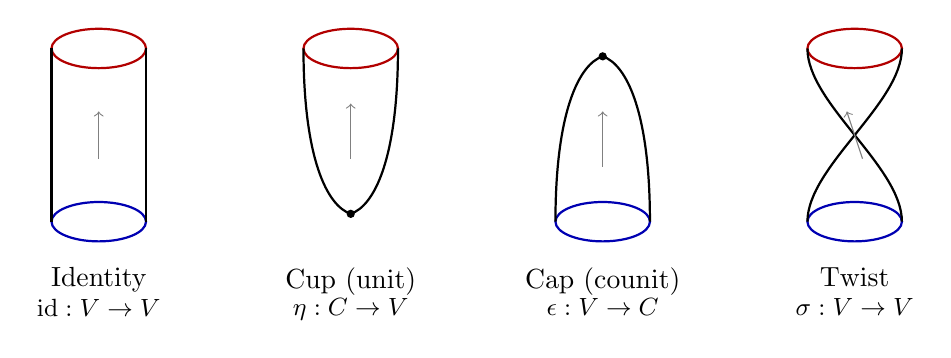
\begin{tikzpicture}[scale=1.0, thick]

  % === Identity cylinder ===
  \begin{scope}[shift={(0,0)}]
    \draw[blue!70!black] (0, 0) ellipse (0.6 and 0.25);
    \draw[red!70!black] (0, 2.2) ellipse (0.6 and 0.25);
    \draw (-0.6, 0) -- (-0.6, 2.2);
    \draw (0.6, 0) -- (0.6, 2.2);
    \draw[->, gray, thin] (0, 0.8) -- (0, 1.4);
    \node[below] at (0, -0.45) {Identity};
    \node[below, font=\small] at (0, -0.85) {$\mathrm{id}: V \to V$};
  \end{scope}

  % === Cup (unit / creation) ===
  \begin{scope}[shift={(3.2, 0)}]
    \draw[red!70!black] (0, 2.2) ellipse (0.6 and 0.25);
    \draw (-0.6, 2.2) .. controls (-0.6, 0.8) and (-0.3, 0.2) .. (0, 0.1);
    \draw (0.6, 2.2) .. controls (0.6, 0.8) and (0.3, 0.2) .. (0, 0.1);
    \fill (0, 0.1) circle (1.5pt);
    \draw[->, gray, thin] (0, 0.8) -- (0, 1.5);
    \node[below] at (0, -0.45) {Cup (unit)};
    \node[below, font=\small] at (0, -0.85) {$\eta: \mathbb{C} \to V$};
  \end{scope}

  % === Cap (counit / annihilation) ===
  \begin{scope}[shift={(6.4, 0)}]
    \draw[blue!70!black] (0, 0) ellipse (0.6 and 0.25);
    \draw (-0.6, 0) .. controls (-0.6, 1.4) and (-0.3, 2.0) .. (0, 2.1);
    \draw (0.6, 0) .. controls (0.6, 1.4) and (0.3, 2.0) .. (0, 2.1);
    \fill (0, 2.1) circle (1.5pt);
    \draw[->, gray, thin] (0, 0.7) -- (0, 1.4);
    \node[below] at (0, -0.45) {Cap (counit)};
    \node[below, font=\small] at (0, -0.85) {$\epsilon: V \to \mathbb{C}$};
  \end{scope}

  % === Twist ===
  \begin{scope}[shift={(9.6, 0)}]
    \draw[blue!70!black] (0, 0) ellipse (0.6 and 0.25);
    \draw[red!70!black] (0, 2.2) ellipse (0.6 and 0.25);
    % Twisted surface: left side crosses to right
    \draw (-0.6, 0) .. controls (-0.6, 0.7) and (0.6, 1.5) .. (0.6, 2.2);
    \draw (0.6, 0) .. controls (0.6, 0.7) and (-0.6, 1.5) .. (-0.6, 2.2);
    \draw[->, gray, thin] (0.1, 0.8) -- (-0.1, 1.4);
    \node[below] at (0, -0.45) {Twist};
    \node[below, font=\small] at (0, -0.85) {$\sigma: V \to V$};
  \end{scope}

\end{tikzpicture}
